\documentclass[class=article, crop=false]{standalone}
\usepackage{graphicx}
\usepackage{tikz}
\usepackage{subcaption}
\usetikzlibrary{calc}
\usepackage{import}

\begin{document}
\begin{minipage}{0.3\linewidth}
    \centering
    \begin{subfigure}{0.45\linewidth}
        \centering
        \documentclass[class=article, crop=false]{standalone}
\usepackage{tikz}
\usepackage{subcaption}
\usetikzlibrary{calc}

\begin{document}
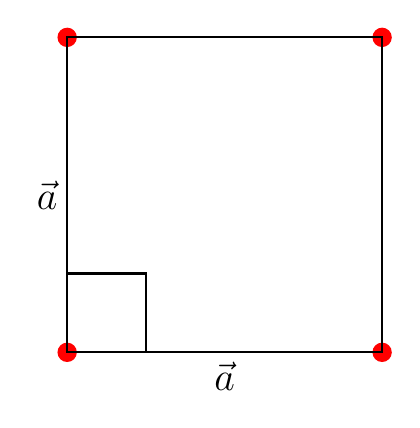
\begin{tikzpicture}
    \def\a{4}  % length of side a

    % Calculate the coordinates of the points
    \coordinate (A) at (0, 0);
    \coordinate (B) at (\a, 0);
    \coordinate (C) at (\a, \a);
    \coordinate (D) at (0, \a);

    \fill[red]  (A) circle(3.5pt) (B) circle(3.5pt) (C) circle(3.5pt) (D) circle(3.5pt);

    % Draw the square unit cell
    \draw[thick] (A) -- (B) -- (C) -- (D) -- cycle;

    % Draw right angle
    \draw[thick] (0,1) -- (1,1) -- (1,0);

    %Draw lattice parameters
    \node[left] at ($(A)!0.5!(D)$) {\Large $\vec{a}$};
    \node[below] at ($(A)!0.5!(B)$) {\Large $\vec{a}$};
    
\end{tikzpicture}
\end{document}
        \caption*{Square Cell}
        \label{fig:square-cell}
    \end{subfigure}
    \vfill
    \begin{subfigure}{0.45\textwidth}
        \centering
        \documentclass[class=article, crop=false]{standalone}
\usepackage{tikz}
\usepackage{subcaption}
\usetikzlibrary{calc}

\begin{document}
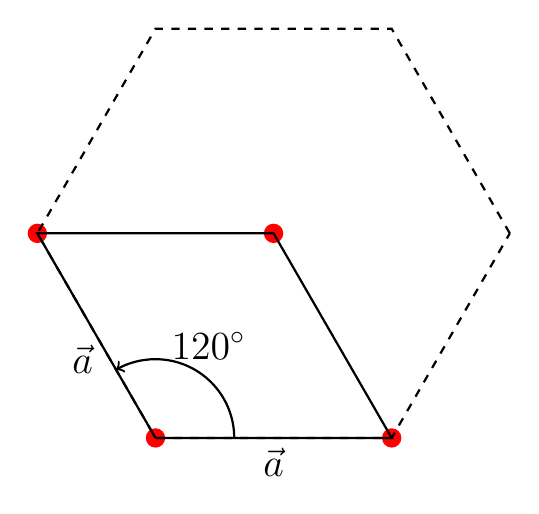
\begin{tikzpicture}
    \def\a{3}  % length of side a

    Calculate the coordinates of the points
    \coordinate (A) at (0:\a);
    \coordinate (B) at (60:\a);
    \coordinate (C) at (120:\a);
    \coordinate (D) at (180:\a);
    \coordinate (E) at (240:\a);
    \coordinate (F) at (300:\a);
    \coordinate (G) at (0,0);


    % Creates nodes at vertices
    \fill[red]  (D) circle(3.5pt) (E) circle(3.5pt) (F) circle(3.5pt) (G) circle(3.5pt);
    

    % Draw the hexagon boundary
    \draw[thick,dashed] (A) -- (B) -- (C) -- (D) -- (E) -- (F) -- (A);

    % Draw the cell
    \draw[thick] (E) -- (F) -- (G) -- (D) -- (E); 

    %Draw lattice parameters
    \node[anchor={60}] at ($(D)!0.5!(E)$) {\Large $\vec{a}$};
    \node[below] at ($(E)!0.5!(F)$) {\Large $\vec{a}$};

    % Optional: add angle markers
    \draw[thick, ->] (E) ++(1,0) arc[start angle=0, end angle=120, radius=1] node[midway,anchor={-120}] {\Large $120^\circ$};
    
\end{tikzpicture}
\end{document}
        \caption*{Hexagon Cell}
        \label{fig:hexagon-cell}
    \end{subfigure}
\end{minipage}
\hspace{2cm}
\begin{minipage}{0.9\linewidth}
    \centering
    \begin{subfigure}{0.45\linewidth}
        \centering
        \documentclass[class=article, crop=false]{standalone}
\usepackage{tikz}
\usepackage{subcaption}
\usetikzlibrary{calc}

\begin{document}

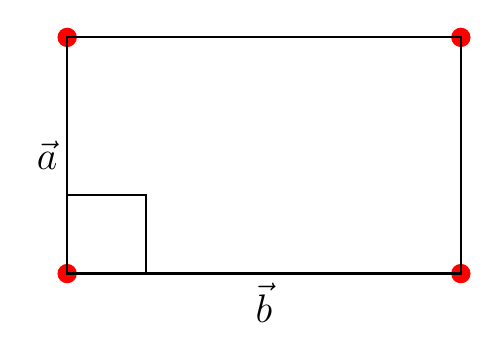
\begin{tikzpicture}
    \def\a{5}  % length of side a
    \def\b{3}  % length of side b
    \def\y{5}

    % Calculate the coordinates of the points
    \coordinate (A) at (0, 0);
    \coordinate (B) at (\a, 0);
    \coordinate (C) at (\a, \b);
    \coordinate (D) at (0, \b);

    %\coordinate (A2) at (0, 0 - \y);
    %\coordinate (B2) at (\a, 0- \y);
    %\coordinate (C2) at (\a, \b - \y);
    %\coordinate (D2) at (0, \b - \y);

    % Creates nodes at vertices
    \fill[red]  (A) circle(3.5pt) (B) circle(3.5pt) (C) circle(3.5pt) (D) circle(3.5pt);% (A2) circle(3.5pt) (B2) circle(3.5pt) (C2) circle(3.5pt) (D2) circle(3.5pt);
    %\fill[blue] ($(A2)!0.5!(C2)$) circle(3.5pt);

    % Draw right angle
    \draw[thick] (0,1) -- (1,1) -- (1,0);
    %\draw[thick] (0,1-\y) -- (1,1-\y) -- (1,0-\y);

    % Draw the rectangular unit cell
    \draw[thick] (A) -- (B) -- (C) -- (D) -- cycle;
    %\draw[thick] (A2) -- (B2) -- (C2) -- (D2) -- cycle;
    %\draw[dashed] (A2) -- (C2);
    %\draw[dashed] (B2) -- (D2);


    %Draw lattice parameters
    \node[left] at ($(A)!0.5!(D)$) {\Large $\vec{a}$};
    \node[below] at ($(A)!0.5!(B)$) {\Large $\vec{b}$};
    %\node[left] at ($(A2)!0.5!(D2)$) {\Large $\vec{a}$};
    %\node[below] at ($(A2)!0.5!(B2)$) {\Large $\vec{b}$};
    
\end{tikzpicture}
        
\end{document}
        \caption*{Rectangle Cell}
        \label{fig:rectangle-cell}
    \end{subfigure}  
    \vfill
    \begin{subfigure}{0.45\linewidth}
        \centering
        \documentclass[class=article, crop=false]{standalone}
\usepackage{tikz}
\usepackage{subcaption}
\usetikzlibrary{calc}

\begin{document}
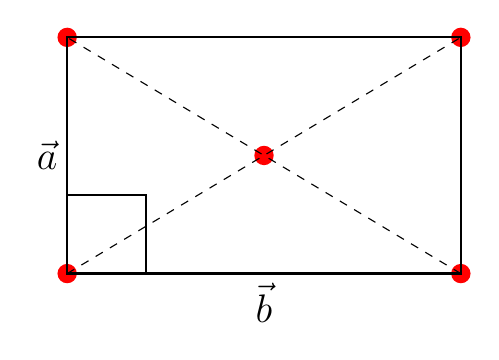
\begin{tikzpicture}
    \def\a{5}  % length of side a
    \def\b{3}  % length of side b

    % Calculate the coordinates of the points
    \coordinate (A) at (0, 0);
    \coordinate (B) at (\a, 0);
    \coordinate (C) at (\a, \b);
    \coordinate (D) at (0, \b);
    %\coordinate (E) at (\a, 2*\b);
    %\coordinate (F) at (0, 2*\b);

    % Creates node labels
    %\node[above left] at (A) {A};
    %\node[above left] at (B) {B};
    %\node[above left] at (C) {C};
    %\node[above left] at (D) {D};
    %\node[above left] at (E) {E};
    %\node[above left] at (F) {F};

    % Creates nodes at vertices
    \fill[red]  (A) circle(3.5pt) (B) circle(3.5pt) (C) circle(3.5pt) (D) circle(3.5pt);% (E) circle(3.5pt) (F) circle(3.5pt);
    % Creates nodes at centers
    \fill[red] ($(A)!0.5!(C)$) circle(3.5pt);
    %\fill[blue] ($(D)!0.5!(E)$) circle(3.5pt);

    % Draw the rectangular unit cell
    \draw[thick] (A) -- (B) -- (C) -- (D) -- cycle;
    %\draw[thick,dashed] (D) -- (F) -- (E) -- (C) -- cycle;
    %\draw[thick] (D) -- ($(A)!0.5!(C)$) -- (C) -- ($(D)!0.5!(E)$) -- cycle;

    % Draw lines
    \draw[dashed] (A) -- (C);
    \draw[dashed] (B) -- (D);

    % Draw right angle
    \draw[thick] (0,1) -- (1,1) -- (1,0);


    %Draw lattice parameters
    \node[left] at ($(A)!0.5!(D)$) {\Large $\vec{a}$};
    \node[below] at ($(A)!0.5!(B)$) {\Large $\vec{b}$};
    
\end{tikzpicture}

\end{document}
        \caption*{Rhombic Cell}
        \label{fig:rhombic-cell}
    \end{subfigure}
    \vfill
    % Oblique
    \begin{subfigure}{0.45\linewidth}
        \centering
        \documentclass[class=article, crop=false]{standalone}
\usepackage{tikz}
\usepackage{subcaption}
\usetikzlibrary{calc}

\begin{document}
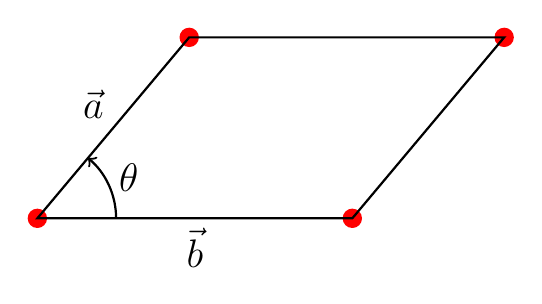
\begin{tikzpicture}
    % Define the lengths of the sides and the angle
    \def\a{4}  % length of side a
    \def\b{3}  % length of side b
    \def\angle{50}  % angle between sides a and b

    % Calculate the coordinates of the points
    \coordinate (A) at (0, 0);
    \coordinate (B) at (\a, 0);
    \coordinate (C) at ({\a + \b*cos(\angle)}, {\b * sin(\angle)});
    \coordinate (D) at ({\b * cos(\angle)}, {\b * sin(\angle)});

    
    % Creates nodes at vertices
    \fill[red]  (A) circle(3.5pt) (B) circle(3.5pt) (C) circle(3.5pt) (D) circle(3.5pt);

    % Draw the oblique unit cell
    \draw[thick] (A) -- (B) -- (C) -- (D) -- cycle;

    %Draw lattice parameters
    \node[anchor={-\angle}] at ($(A)!0.5!(D)$) {\Large $\vec{a}$};
    \node[below] at ($(A)!0.5!(B)$) {\Large $\vec{b}$};
    
    % Optional: add angle markers
    \draw[thick, ->] (A) ++(1,0) arc[start angle=0, end angle=\angle, radius=1] node[midway, anchor={150+\angle}] {\Large $\theta$};
\end{tikzpicture}
\end{document}
        \caption*{Oblique Cell}
        \label{fig:oblique-cell}
    \end{subfigure}
\end{minipage}

\end{document}